\chapter{Construirea unei suite de aplicații pentru evaluarea 
tehnicilor de testare}

După cum am argumentat în capitolele precedente, sistemele \acrshort{iot} sunt complexe, eterogene și distribuite, caracteristici care aduc o serie de dificultăți greu de depășit în testare. Am oferit o argumentare detaliată asupra acestor aspecte în secțiunea \textbf{2.2.Q3}. Pentru a avansa în ce privește starea curentă a tehnicilor de testare, avem nevoie de metrici \footnote{În acest context, „metrici” se referă la metode de măsurare a rezultatelor unor experimente.} obiective, care ar ușura munca cercetătorilor de a reproduce rezultate și de a le compara. În urma analizei literaturii din secțiunea \textbf{2.2.Q4}, am constatat imposibilitatea stabilirii unor astfel de metrici, deoarece majoritatea publicațiilor utilizează o suită proprie de aplicații pentru desfășurarea experimentelor. Astfel, a compara numărul de defecte descoperite, timpul sau alți parametri este irelevant, deoarece mediul variază. 

Regăsim aceeași concluzie enunțată de \citet{Paduraru2021}, în articolul lor, care propune o specificație formală pentru descrierea sistemelor \acrshort{iot}. Pentru evaluarea riguroasă a specificației propuse este nevoie de construirea unei suite de aplicații cât mai apropiate de realitate. Această inițiativă este materializată și prezentată de lucrarea lui \citet{Cristea2022}. Aceasta va fi prezentată în paginile ce urmează, evidențiind contribuțiile proprii.

Un aspect important al suitei de aplicații construit este faptul că este \textit{open-source}. Într-o industrie în care majoritatea producătorilor nu pun la dispoziție decât sursele deja compilate ale \textit{firmware}-ului, iar în multe cazuri acestea se află pe dispozitive ce nu permit accesarea lui, existența \textit{software}-ului \textit{open-source} este crucială pentru a crea un mediu transparent pentru experimente.

O observație importantă este că suita de aplicații este realizată în mare măsură imitând aplicațiile reale dintr-o locuință inteligentă, deoarece este unul din cele mai întâlnite scenarii de utilizare a tehnologiilor \acrshort{iot}, și pentru că oferă un grad de complexitate și interconectare suficient de mic încât să fie realizat fără eforturi majore, dar și suficient de mare, încât să mimeze comportamentul unui sistem real, aducând același tip de provocări.

În prezentul capitol, vom discuta despre modul de construire al suitei de aplicații și particularitățile fiecărei aplicații în parte, prezentând funcționalitatea și tehnologiile utilizate pentru realizarea ei. Apoi, ne vom concentra asupra infrastructurii de interconectare a aplicațiilor și vom discuta despre protocoalele utilizate și motivația alegerii lor. Pentru a ilustra o situație cât mai apropiată de realitate, aplicațiile sunt angrenate în fluxuri de automatizări orchestrate de o unitate centrală, analiza acestor fluxuri fiind de asemenea prezentă în acest capitol. După înțelegerea structurală a setului de aplicații, vom vedeam cum îl putem folosi pentru compararea și analizarea tehnicilor de testare și cum poate fi acesta util pentru cercetători sau profesioniști. În final, ne vom concentra asupra limitărilor și posibilelor îmbunătățiri ce ar putea fi aduse în viitor setului de aplicații.

\section{Descrierea aplicațiilor}

Pentru a ilustra cât mai bine o situație reală, aplicațiile utilizate au surse multiple, o parte fiind dezvoltate de echipe independente de studenți, o altă parte au fost scrise de echipa de cercetare \acrshort{sasha}, iar altele au fost obținute din surse publice. Au fost aduse modificări pentru a facilita integrarea, dar și pentru a introduce defecte (\textit{en. bugs}) artificiale pe lângă cele deja existente. Această diversitate se regăsește și în sectorul comercial, acolo unde dispozitive și software de la producători diferiți sunt utilizate în medii complexe și condiții impredictibile. Considerăm că această abordare de construire a aplicațiilor este suficient de robustă și suficient de apropiată de realitate.

În paragrafele următoare, vom analiza caracteristicile fiecărei aplicații \footnote{Codul sursă al aplicațiilor, infrastructura și documentația acestora pot fi găsite la \url{https://github.com/unibuc-cs/IoT-application-set}.}, caracteristici precum modul de funcționare, tehnologiile utilizate pentru dezvoltare, dependența și interacțiunea față de alte aplicații sau relevanța pentru evaluarea tehnicilor de testare. Toate aplicațiile simulează procese des întâlnite în locuințele inteligente.

% ===================================================================== DONE
\subsection*{FlowerPower}

\textbf{Descriere}:  Un \textit{ghiveci inteligent} care expune prin intermediului unui \acrshort{api} supravegherea și îngrijirea plantelor. De asemenea, poate notifica utilizatorul în legătură cu anumite schimbări legate de starea plantelor.

\textbf{Tehnologii utilizate}: \textit{C++} și \textit{GNU Makefiles} pentru dezvoltare, împreună cu bibliotecile \textit{Pistache} pentru servirea de cereri \acrfull{http}, \textit{RapidJson} pentru lucrul cu date în format \acrfull{json} și \textit{Mosquitto} pentru comunicarea cu un distribuitor de mesaje prin protocolul \acrfull{mqtt}. 

\textbf{În context}: Interacționează cu aplicația WindWow în legătură cu aspecte precum temperatura sau luminozitatea.

\textbf{Sursă}: Echipă de Studenți înscriși la cursul de Ingineria Programării, anul 2020.
% =====================================================================

% =====================================================================
\subsection*{WindWow}

\textbf{Descriere}:  O fereastră inteligentă ce permite monitorizarea temperaturii și luminozității din cameră, luminozitatea fiind reglabilă prin intermediul draperiilor acționate de utilizator de la distanță.

\textbf{Tehnologii utilizate}: \textit{C++} și \textit{CMake} pentru dezvoltare, împreună cu bibliotecile \textit{Pistache}, \textit{NLohmann-JSON} pentru lucrul cu date în format \acrshort{json} și \textit{Mosquitto}.

\textbf{În context}: Senzorii de luminozitate și temperatură colectează date relevante pentru o multitudine de alte dispozitive din rețea, cum ar fi SmartFlower și SmartTV, care își pot calibra funcționarea în funcție de datele primite.

\textbf{Sursă}: Echipă de Studenți înscriși la cursul de Ingineria Programării, anul 2020.
% =====================================================================

% =====================================================================
\subsection*{Smarteeth}

\textbf{Descriere}: O periuță electrică ce permite colectarea de statistici de sănătate și multiple programe de utilizare.

\textbf{Tehnologii utilizate}: \textit{C++} și \textit{CMake} pentru dezvoltare, \textit{Paho} pentru lucrul cu date în format \acrshort{json} și \textit{Mosquitto}.

\textbf{În context}: Dispozitivul este relativ izolat, interacționează minimal, doar cu SmartKettle.

\textbf{Sursă}: Echipă de Studenți înscriși la cursul de Ingineria Programării, anul 2020.
% =====================================================================

% =====================================================================
\subsection*{SmartKettle}

\textbf{Descriere}: Fierbător inteligent dotat cu senzori pentru temperatură și vâscozitate, poate fi programat pentru a prepara băuturi în mod recurent.

\textbf{Tehnologii utilizate}: \textit{C++}, \textit{Bash scripting}, \textit{Makefiles}, \textit{NLohmann-JSON} și \textit{Pistache}.

\textbf{În context}: Preia date legate de temperatură de la WindWow pentru a determina temperatura de preparare a băuturilor.

\textbf{Sursă}: Echipă de Studenți înscriși la cursul de Ingineria Programării, anul 2020.
% =====================================================================

% =====================================================================
\subsection*{SmartTV}

\textbf{Descriere}: TV inteligent, programabil, dotat cu sistem de recomandări personalizabil pentru fiecare utilizator.

\textbf{Tehnologii utilizate}: \textit{C++}, \textit{CMake}, \textit{NLohmann-JSON} și \textit{Pistache}.

\textbf{În context}: Își reglează luminozitatea conform datelor primite de la senzorii aplicației WindWow.

\textbf{Sursă}: Echipă de Studenți înscriși la cursul de Ingineria Programării, anul 2020.
% =====================================================================

% =====================================================================
\subsection*{SeraSmart}

\textbf{Descriere}: Seră inteligentă pentru îngrijirea plantelor asistată de computer, dotată cu senzori similari cu cei ai aplicației FlowerPower.

\textbf{Tehnologii utilizate}: \textit{Python 3.7}, \textit{Flask} pentru \textit{server}-ul \acrshort{http}, \textit{PyYAML}, \textit{Mosquitto} și \textit{SQLite}.

\textbf{Sursă}: Echipă de Studenți înscriși la cursul de Ingineria Programării, anul 2021.
% =====================================================================

% =====================================================================
\subsection*{SoundSystem}

\textbf{Descriere}: Music player programabil, cu acces la internet și spațiu de stocare propriu.

\textbf{Tehnologii utilizate}: \textit{Golang} pentru dezvoltare, \textit{Echo Library} pentru \textit{server}-ul \acrshort{http} și \textit{Paho}.

\textbf{În context}: Preia comenzi directe de la utilizatori și informează aplicația Hub despre starea sa curentă.

\textbf{Sursă}: Autorul prezentei lucrări
% =====================================================================

% =====================================================================
\subsection*{PhilipsHue Simulator}

\textbf{Descriere}: O aplicație formată din mai multe componente: leduri, becuri, un TV și \textit{hub}-uri de sincronizare. Simulează jocul de lumini al unui sistem PhiliphsHue.

\textbf{Tehnologii utilizate}: \textit{Python}, \textit{Rust} și \textit{Cargo} pentru dezvoltare, \textit{warp} pentru \textit{server}-ul \acrshort{http}.

\textbf{În context}: TV-ul comunică date despre videoul afișat spre HDMIBox, acesta procesându-le și trimițându-le mai departe la PhiliphsHub. \textit{Hub}-ul va sincroniza celelalte dispozitive luminoase (leduri, becuri etc.), astfel încât jocul de lumini este în armonie cu videoul.

\textbf{Sursă}: Autorul prezentei lucrări
% =====================================================================

Observăm ca aplicațiile prezentate sunt variate atât din punct de vedere al tehnologiilor utilizate (\textit{C++}, \textit{Python}, \textit{Go}, \textit{Rust}), cât și din punct de vedere al funcționării lor, acestea acoperind o gamă largă de utilizări posibile în cadrul unei locuințe inteligente. 

În secțiunea următoare vom prezenta modul în care aceste aplicații au fost integrate într-o suită coerentă cu fluxuri de intercomunicare complexe.

\section{Infrastructura}

\begin{figure}[h]
    \centering
    \caption{\centering Infrastructura parțială a suitei de aplicații. În centrul rețelei se află aplicația Hub care orchestrează comunicațiile dintre celelalte aplicații. Lateral sunt menționate tehnologiile utilizate pentru \textit{deployment} (Docker, RaspberryPi) și specificații (OpenAPI, AsyncApi).}
    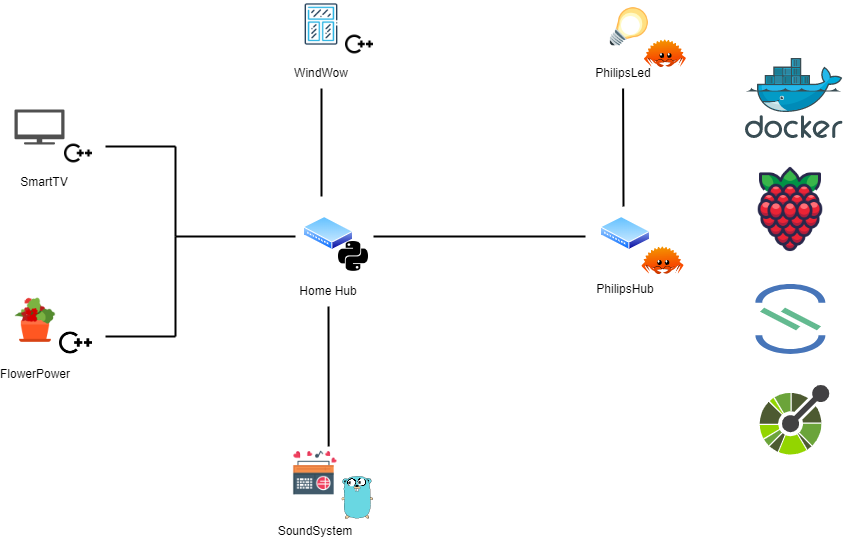
\includegraphics[width=0.9\textwidth]{images/smarthome_dataset.drawio (1).png}
    \label{fig:app_dataset_infra}
\end{figure}

\begin{figure}[h]
    \centering
    \caption{\centering Ilustrarea unui flux de automatizare. Aplicația WindWow comunică aplicației Hub o luminozitate scăzută, așa că aplicația Hub va ajusta luminozitatea aplicației SmartTV și va porni lampa asociată aplicației FlowerPower.}
    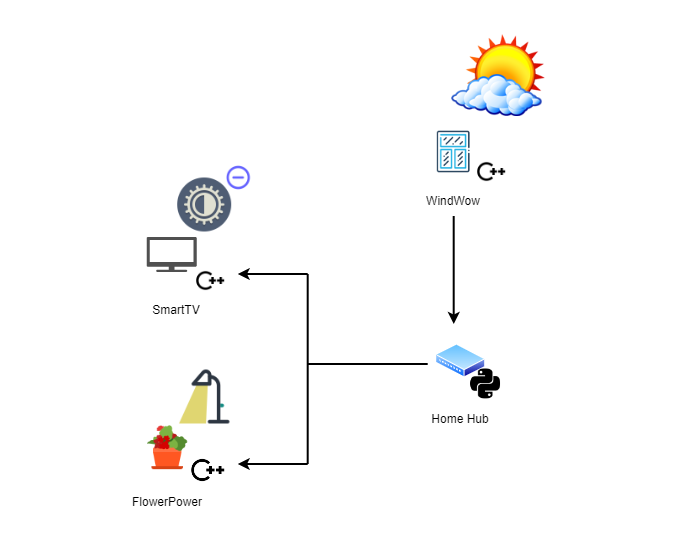
\includegraphics[width=0.9\textwidth]{images/smarthome_automation.drawio (2).png}
    \label{fig:app_flux}
\end{figure}

Așa cum am menționat anterior, dispozitivele dintr-un sistem \acrshort{iot} sunt interconectate și fac parte din fluxuri de complexități variate. Pentru a ne păstra cât mai aproape de un sistem real, aplicațiile mai sus menționate au fost puse într-o rețea comună și orchestrate folosind o aplicație centrală, în general cunoscută sub numele de \textit{hub}. Rețeaua poate fi desfășurată (en. \textit{deployed} - \textit{deployment}) atât într-un mediu virtualizat, folosind tehnologiile \textit{Docker} și \textit{docker-compose}, dar și într-un mediu cu hardware fizic folosind o serie de \textit{script}-uri de automatizare, dar și câteva operații manuale. În experimentele desfășurate, am folosit atât mediul virtualizat, cât și un \textit{deployment} pe arhitectura \textit{x86} \footnote{Arhitectură comună pentru computerele de uz personal, folosită de brand-uri precum Intel și AMD.} și pe \textit{ARMv7l}, \footnote{Arhitectură utilizată pentru dispozitive mici și portabile cum ar fi telefoanele mobile, întâlnită des și în IoT.} folosind un \textit{Raspberry Pi 2 Model B}. În figura \ref{fig:app_dataset_infra}, putem observa câteva din aplicațiile descrise mai sus și topologia rețelei care le pune împreună.

Punctul central al rețelei este reprezentat de aplicația \textit{hub}. Aceasta este responsabilă cu monitorizarea și orchestrarea tuturor dispozitivelor din rețea și permite implementarea fluxurilor de automatizare. Un astfel de flux poate fi observat în figura \ref{fig:app_flux}, unde avem prezentată sincronizarea luminozității mai multor dispozitive pe baza datelor colectate de aplicația WindWow. 

\textit{Hub}-ul este o aplicație proprie dezvoltată cu limbajul \textit{Python} și permite integrarea a două protocoale de comunicație în momentul de față: \acrshort{http} și \acrshort{mqtt}. Am ales să nu folosim o aplicație \textit{hub} comercială cum ar fi \textit{OpenHAB} sau \textit{Home Assistant}, deoarece avantajele aduse de o soluție personalizată din punct de vedere al timpului de integrare și al simplității au fost superioare.

Pentru a asigura omogenitatea comunicării într-un sistem cu componente eterogene, toate aplicațiile au specificații \textit{OpenAPI} \footnote{Specificație bazată pe limbajul \acrshort{yaml} care poate descrie modul de autentificare, verbele și rutele unui \acrshort{api} bazat pe protocolul \acrshort{http}. Mai multe detalii pot fi găsite la adresa \url{https://swagger.io/specification/}.} pentru descrierea rutelor \acrshort{http} expuse și specificații \textit{AsyncAPI} \footnote{Specificație construită peste OpenAPI, aceasta fiind orientată spre descrierea de sisteme \acrshort{eda}. Mai multe informații pot fi găsite la adresa \url{https://www.asyncapi.com/}.} pentru descrierea formatului mesajelor transmise prin intermediul protocolului \acrshort{mqtt}. Folosind \textit{OpenAPI Generator} \footnote{Utilitar software care transformă specificații OpenAPI în cod sursă în diferite limbaje de programare. Utilitarul poate fi găsit la \url{https://openapi-generator.tech/}.}, specificațiile \textit{OpenAPI} pot fi transformate în cod de interacțiune cu aplicațiile. Codul generat a fost utilizat în aplicația de \textit{hub}, pentru a oferi acces uniform la aplicații.

Față de protocolul \acrshort{http}, protocolul \acrshort{mqtt} operează în manieră \textit{publisher}/\textit{subscribe}, nu \textit{request}/\textit{reqsponse}, astfel devine necesară existența unui distribuitor de mesaje în rețea. Pentru această sarcină am utilizat \textit{Eclipse Mosquitto}, deoarece este un produs \textit{open-source} ușor de instalat și folosit atât în mediu virtualizat, cât și nevirtualizat.

Întreaga configurație este stocată în câteva fișiere în format, \acrfull{yaml} sau \acrshort{json}, aceasta specificând numele și calea aplicațiilor, porturile de rețea expuse și alți parametri specifici. De asemenea, conține informații despre aplicația \textit{hub} și serviciile externe necesare (cum ar fi distribuitorul de mesaje). Configurația este citită de utilitarele construite pentru a facilita cele mai comune operații: compilarea aplicațiilor, rularea aplicațiilor pe mediul local, virtualizat sau nu, executarea unor teste, repornirea sau oprirea aplicațiilor, instalarea dependințelor software, etc.

\textit{Docker} este o soluție software pentru izolarea aplicațiilor în containere. Față de mașinile virtuale clasice care fie utilizează facilitățile de virtualizare ale unității centrale de procesare, fie emulează în întregime o unitate centrală, \textit{Docker} pune la dispoziție un strat de abstractizare între aplicații și sistemul de operare, astfel încât acestea se execută într-un mediu izolat denumit container, fără acces la restul sistemului. De asemenea, configurarea dependințelor și mediului din container în care va fi executată aplicația sunt specificate în mod textual, în așa numitele \textit{Dockerfiles}. Această abordare aduce o serie de avantaje printre care se numără o mai bună securitate pentru un cost mic de performanță și o bună reproductibilitate a mediilor. Pentru a orchestra mai multe containere, folosim \textit{docker-compose} care poate fi configurat în mod textual. Acesta permite și configurarea de topologii, medii de stocare și interacțiunea cu sistemul gazdă.

Utilizarea suitei de aplicații în containere de tip \textit{Docker} este convenientă, deoarece consumă puține resurse și nu necesită pregătiri suplimentare, însă pentru a simula un scenariu mai apropiat de realitate, aplicațiile pot fi puse pe dispozitive hardware fizice cum ar fi \textit{Raspberry Pi}. Am pus la dispoziție scripturile necesare pentru compilarea aplicațiilor și instalarea dependințelor pentru un sistem \textit{Raspbian ARMv7l}. Aplicațiile împreună cu \textit{hub}-ul și distribuitorul de mesaje au fost desfășurate pe mai multe \textit{Raspberry Pi's} conectate prin \textit{wi-fi}.

\section{Extinderea suitei de aplicații}

Deoarece există un număr foarte mare de posibile tipuri de sisteme \acrshort{iot} și utilizări ale acestora, suita de aplicații nu acoperă decât un mic număr din total. Astfel, încurajăm extinderea și îmbogățirea suitei cu aplicații și fluxuri de automatizare proprii atât din partea cercetătorilor, cât și a profesioniștilor. Pașii pentru includerea unei noi aplicații sunt simplii și puțini la număr, astfel asigurând un proces cât mai puțin anevoios. În rândurile ce urmează, vom parcurge ce caracteristici trebuie sa aibă o nouă aplicație și ce pași trebuie urmați pentru includerea ei.

\textbf{Caracteristici necesare}:
\begin{enumerate}
    \item Aplicația trebuie să comunice folosind cel puțin unul din protocoalele \acrshort{http} sau \acrshort{mqtt}.
    \item Sunt necesare specificații \textit{OpenAPI} și/sau \textit{AsyncAPI}, în funcție de protocoalele folosite.
    \item Codul trebuie să poată fi compilat pentru arhitectura \textit{x86} sau să poată fi cel puțin executat într-un emulator.
\end{enumerate}

\textbf{Integrarea în suită} \footnote{Tutorialul complet poate fi găsit la adresa \url{https://github.com/unibuc-cs/IoT-application-set/blob/master/HOW_TO_ADD_AN_APP.md}.}:
\begin{enumerate}
    \item Crearea configurațiilor necesare pentru generarea de clienți de comunicare (momentan doar pentru \acrshort{http}).
    \item Punerea la dispoziție a unui \textit{script} de instalare al dependințelor aplicației.
    \item Punerea la dispoziție a unui \textit{script} de compilare a aplicației, pentru arhitecturile țintă.
    \item Punerea la dispoziție a unui \textit{script} pentru executarea aplicației pe un port de rețea arbitrar.
    \item Crearea unei configurații în format \textit{Dockerfile} și adăugarea unei intrări în configurația generală a suitei.
    \item Copierea codului sursă a noii aplicații în directorul corespunzător.
\end{enumerate}

Deși recomandăm integrarea aplicațiilor \textit{open-source}, în cazul în care sursa nu este disponibilă, se pot omite pașii de compilare și copiere a sursei aplicației. Este necesar să ne asigurăm că binarele puse la dispoziție pot fi executate pe arhitectura \textit{x86}, fie direct, fie prin intermediul unui emulator.

\section{Defecte, evaluare și limitări}

Scopul suitei de aplicații este compararea metodelor de testare, așa cum am menționat anterior. Pentru a oferi un reper relevant, este necesar ca aplicațiile să conțină defecte realiste. Cum aceste aplicații au fost dezvoltate de multiple echipe de studenți, conțin în mod natural o serie de defecte, defecte pe care le-am identificat în urma testării funcționale a suitei, dar despre acest proces vom discuta în capitolul următor. Pe lângă defectele existente, am considerat necesară îmbogățirea suitei cu o gamă mai largă de defecte. Acestea au fost introduse în codul aplicațiilor sau în regulile de automatizare din aplicația \textit{hub}, unele defecte fiind o combinație din ambele.

Deoarece una din caracteristicile principale ale \acrshort{iot} este numărul mare de părți comunicante, am ales să împărțim defectele descoperite și injectate în trei categorii bazate pe nivelul de interacțiune dintre părțile sistemului. Aceste categorii sunt următoarele:

\begin{enumerate}
    \item Defecte la nivel de aplicație - acestea afectează doar aplicații individuale, efectele comune fiind funcționarea incorectă sau oprirea funcționării în totalitate.
    \item Defecte la nivel de flux de automatizare - caracterizate de rezultatul incorect la finalul executării unui singur flux de automatizare ce conține multiple aplicații.
    \item Defecte la nivel de persistență în sistem - atunci când execuția a mai multor fluxuri de automatizare care nu sunt disjuncte duce la funcționarea incorectă a întregului sistem.
\end{enumerate}

\begin{figure}[h]
    \centering
    \caption{\centering Cele trei niveluri de defecte reprezentate în ordinea complexității acestora.}
    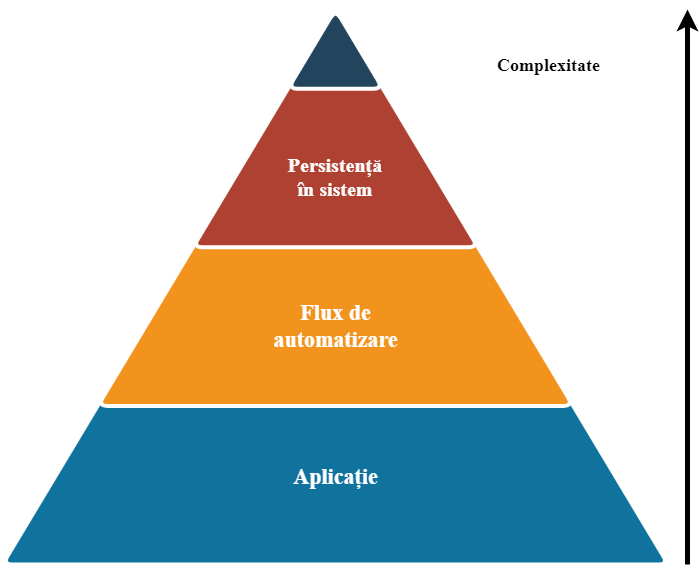
\includegraphics[width=0.6\textwidth]{images/niveluri_defecte.drawio (1).png}
    \label{fig:bug_levels}
\end{figure}

În general, defectele din prima categorie au fost cel mai des abordate în literatură, majoritatea soluțiilor existente concentrându-se pe acestea. Pe de altă parte, defectele din celelalte categorii au un grad de dificultate de detectare mult mai ridicat, deoarece sunt cauzate, în general, de concurență și sunt în strânsă legătură cu domeniul specific în care este utilizată aplicația. Să luăm un exemplu pentru a ne face o imagine mai clară, un defect din categoria întâi poate fi reprezentat de un acces invalid de memorie care cauzează un răspuns întârziat, un răspuns cu date aleatorii sau chiar nefuncționarea completă a aplicației. Metricile de detectare sunt clare și independente de logica concretă a aplicației. Un defect din categoria a treia este mult mai subtil și dificil de detectat. Spre exemplu, să considerăm că un senzor de lumină inteligent determină acționarea draperiilor în funcție de nivelul de luminozitate înregistrat. Utilizatorul comandă manual draperiile, în timp ce acestea sunt în curs de acționare și cauzează blocarea mecanismului. În acest caz, detectarea defectului nu mai este la fel de evidentă, iar producerea acestuia necesită suprapunerea mai multor evenimente independente. 

În studiul realizat de \citet{Zhou2021}, se menționează o clasă de defecte cauzate de acțiuni impredictibile în cadrul fluxurilor de automatizări. Această clasă de defecte este ceea ce noi considerăm a fi defectele de nivel doi și trei în categorisirea proprie. Conform autorilor studiului, cauzele acestei clase de defecte sunt următoarele:

% TODO: cum zic race condition in romana?
\begin{enumerate}
    \item \textit{race condition} între diferite fluxuri;
    \item evenimente lipsă sau procesate într-o ordine imprevizibilă;
    \item acțiuni duplicate sau în conflict.
\end{enumerate}

% În lucrarea de față am ales însă să împărțim defectele în trei categorii în funcție de numărul de componente angrenat în reproducerea defectului. Acest lucru a fost motivat de natura sistemelor \acrshort{iot}, unde interconectarea unui număr mare de dispozitive este des întâlnită. Avem astfel în figura \ref{fig:bug_levels} reprezentarea acestor categorii. Defectele la nivel de aplicație sunt cele care implică o singură aplicație și sunt în general legate de utilizarea incorectă a memoriei. Defectele la nivel de flux de automatizare sunt defecte de concurență care angrenează mai multe aplicații în interiorul aceluiași flux de automatizare. În final, defectele de persistență în sistem sunt cele care sunt produse de intersectarea neașteptată a mai multor fluxuri de automatizare.

În rândurile de mai jos, vom analiza câteva exemple de defecte existente și introduse din toate cele trei categorii numite \footnote{O listă completă a defectelor și codului aferent acestora poate fi găsită la \url{https://github.com/unibuc-cs/IoT-application-set/tree/master/bug_unpatches}.}. De asemenea, vom prezenta liniile de program responsabile pentru producerea defectului, alături de modul în care acesta poate fi rezolvat. Secțiunile de cod vor fi reprezentate folosind formatul \textit{diff} \footnote{Format introdus de utilitarul POSIX \textit{diff} care permite vizualizarea diferențelor între fișiere text prin prefixarea liniilor cu simboluri care reprezintă adăugarea, ștergerea sau modificarea. Colorarea liniilor aduce un plus vizibilității.}. În cadrul suitei de aplicații, toate defectele sunt reparate, însă acestea pot fi activate selectiv folosind capabilitățile de \textit{patching} ale utilitarului \textit{git}.

În aplicația WindWow, am introdus un defect artificial care cauzează un acces al unei adrese invalide de memorie. Acesta este declanșat atunci când draperiile sunt trase și încercăm să setăm o luminozitate mai mare de 25.

\begin{lstlisting}[language=diff, caption={Accesarea adresei nule va cauza oprirea aplicației WindWow}]
--- a/apps/windwow/Window.cpp
+++ b/apps/windwow/Window.cpp
@@ -115,10 +115,9 @@ class Window {
                     if(settings[i].name == "luminosity") {
                         if(settings[i].value > 25.0) {
                             if(changed_state[3] % 2 == 0) {
-                                // BUG TO UNPATCH
                                 // START FAKE BUG
-                                // volatile int *p = nullptr;
-                                // p[50] = 0xdeadbeef;
+                                volatile int *p = nullptr;
+                                p[50] = 0xdeadbeef;
                                 // END FAKE BUG
\end{lstlisting}

Un defect găsit în aplicația SmartPot este lipsa validărilor asupra datelor primite de la utilizatori. Aplicația folosește formatul \acrshort{json} pentru primirea cererilor. Datele din aceste cereri sunt reprezentate în memorie prin intermediul unui dicționar (tabel de dispersie, \textit{hash-map}). Aplicația nu validează existența cheilor accesate atunci când primește o cerere de actualizare a setărilor, astfel cauzând nefuncționarea aplicației.

\begin{lstlisting}[language=diff, caption={Lipsa validării cheilor JSON în aplicația SmartPot}]
--- a/apps/flowerpower/src/SmartPotEndpoint.cpp
+++ b/apps/flowerpower/src/SmartPotEndpoint.cpp
@@ -269,8 +269,7 @@ namespace pot
         double sensorMax = document["max"].GetDouble();
 
         // Valoarea o updatam in MQTT.
-        // BUG TO UNPATCH don't check for HasMember
-        if ((!document.HasMember("nutrientType")) or
-            document["nutrientType"].IsNull())
+        if (document["nutrientType"].IsNull())
         {
             Sensor aux = smartPot->GetSensor(sensorNameMap[sensorTypeID]);
             aux.SetMinValue(sensorMin);
\end{lstlisting}

Unul din defectele introduse la nivel de flux de automatizare este sanitizarea \footnote{Neologism, tradus din engleză, \textit{to sanitize} - \textit{sanitization}. În context, se referă la curățarea datelor posibil malițioase. O traducere inexactă, dar ad litteram este \textit{sanitization} = \textit{sanitație}.} insuficientă a datelor transmise spre SmartTV. Cum am văzut în secțiunea precedentă, există un flux de automatizare care reglează luminozitatea SmartTV-ului, în funcție de datele colectate de la aplicația WindWow. SmartTV-ul acceptă valori de luminozitate în intervalul $(1, 10)$, însă aplicația \textit{hub} poate trimite valori în afara acestuia, cauzând eșecul cererii de actualizare.

\begin{lstlisting}[language=diff, caption={Valorile luminozității transmise spre SmartTV nu sunt doar în intervalul (1, 10)}]
--- a/hub/app.py
+++ b/hub/app.py
@@ -181,8 +181,6 @@ def rule4(env: Environment):
             10 - env.data["windwow"]["luminosity"]/10 + brightness_base,
             brightness_base 
         )
-    # // BUG TO UNPATCH forget to call min
-    env.data["smarttv"]["brightness"] = min(
-       env.data["smarttv"]["brightness"], 
-       10)
     env.clients["smarttv"].set_brightness_level_post(
        int(env.data["smarttv"]["brightness"])
    )
\end{lstlisting}

Intersectarea dintre două fluxuri de automatizare legate de WindWow și FlowerPower cauzează un defect din categoria a treia, anume defecte la nivel de persistență. Așa cum am văzut în cazul unei temperaturi prea ridicate, luminozitatea va fi redusă prin acționarea draperiilor, însă acest eveniment poate declanșa aprinderea lămpii FlowerPower în mod nenecesar, astfel încălzind excesiv planta. 

\begin{lstlisting}[language=diff, caption={Lipsa verificării temperaturii cauzează un conflict între două fluxuri de automatizare}]
--- a/hub/app.py
+++ b/hub/app.py
@@ -165,8 +165,7 @@ def rule3(env: Environment):
     luminosity_sensor_id = 3
     threshold = env.settings["plant_lamp_window_treshold"]
 
-    # // BUG TO UNPATCH don't check window temperature
-    if env.data["windwow"]["luminosity"] < threshold and 
-        env.data["windwow"]["temperature"] < 30:
+    if env.data["windwow"]["luminosity"] < threshold:
         env.clients["flowerpower"].activate_solar_lamp_get()
\end{lstlisting}

Pentru a evalua o tehnică sau o unealtă de testare folosind suita de aplicații, putem activa selectiv defectele sau tipurile de defecte asupra cărora suntem interesați. În urma aplicării metodologiei ce se dorește a fi evaluată, putem colecta o serie de metrici ce vor servi ca mijloc de comparare cu alte metodologii. Câteva posibile astfel de metrici sunt timpul și numărul de defecte descoperite, ratele de detecție per categoria de defecte sau acoperirea codului sau a stărilor posibile ale sistemului. Rămâne la latitudinea cercetătorilor să decidă care sunt cele mai potrivite metrici pentru evaluarea metodologiei în cauză și să interpreteze rezultatele. Oferirea unei metodologii de alegere a experimentelor de evaluare este în afara scopului acestei lucrări.

Deși defectele introduse sunt comparabile cu cele existente în realitate și pot oferi un punct de plecare pentru analiza tehnicilor de testare, trebuie să luăm în considerare și limitările acestei suite de aplicații. Un punct slab este reprezentat de lipsa software-ului găsit pe dispozitive reale, aplicațiile curente fiind simulări ale unor procese reale. De asemenea, acestea sunt proiectate să funcționeze în principal doar pe sisteme a căror arhitectură suportă un sistem de operare compatibil cu \acrfull{posix} sau similar, pe când în realitate multe dispozitive nu au un sistem de operare. În plus, suita conține un număr mic de protocoale de comunicație (doar \acrshort{http} și \acrshort{mqtt}). Toate aceste limitări vor fi adresate în viitoarele activități de cercetare.

Acum, după ce am construit o suită de aplicații care să fie similară unui sistem dintr-o locuință inteligentă cu fluxuri de automatizări și comunicare între dispozitive prin protocoale specifice, vom continua în capitolul următor prin aplicarea câtorva metodologii și unelte de testare. Vom folosi defectele prezentate pentru a compara aceste metodologii și pentru a putea analiza avantajele și dezavantajele acestora în raport cu metricile de evaluare alese.